% !TeX encoding = UTF-8
% !TeX program = PdfLaTeX

\documentclass[UTF8,a6paper]{ctexart}
\usepackage{graphicx} % includegraphics
\usepackage{cite} % citation
\usepackage{float} % [H]
\usepackage{geometry}
\geometry{a6paper,centering,scale=0.8}
\usepackage[nottoc]{tocbibind} % add bib to tableofcontents

\title{\heiti 杂谈勾股定理}
\author{\kaishu 张三}
\date{2010年11月5日}

\newtheorem{theorem}{定理}

\begin{document}

\maketitle
\begin{abstract}
这是一篇关于勾股定理的小短文。
\end{abstract}
\tableofcontents

\newpage
\section{勾股定理在古代}
\label{sec:ancient}
西方称勾股定理为毕达哥拉斯定理,将勾股定理的发现归功于公元前 6 世纪的毕达哥拉斯学派\cite{kline_gujinshuxue_2002}。该学派得到一个法则,可以求出可以排成直角三角形三边的三元数组。毕达哥拉斯学派没有书面著作,该定理的严格表述和证明则见于欧几里德\footnote{欧几里德,约公元前 330--275 年}《几何原本》的命题 47:“直角三角形斜边上的正方形等于两只脚边上的两个正方形之和。”证明是用面积做的。

我国《周髀算经》载商高(约公元前 12 世纪)答周公问:
\begin{quote}
\zihao{-5}\kaishu 勾广三,股修四,径隅五。
\end{quote}

又载陈子(约公元前 7--6 世纪)答荣方问:
\begin{quote}
\zihao{-5}\kaishu 若求邪至日者,以日下为勾,日高为股,勾股各自乘,并而开方除之,得邪至日。
\end{quote}
都较古希腊更早。后者已经明确道出勾股定理的一般形式。图 \ref{fig:xiantu} 是我国古代对勾股定理的一种证明\cite{quanjing_gougu_1998}。
\begin{figure}[ht]
\centering
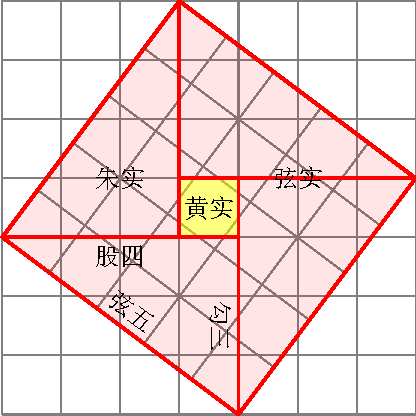
\includegraphics[width=3cm]{fig/xiantu.pdf}
\caption{\small\it 宋赵爽在《周髀算经》注中作的弦图(仿制),该图给出了勾股定理的极具对称美的证明。}
\label{fig:xiantu}
\end{figure}


\section{勾股定理的现代形式}
勾股定理可以用现代语言表述如下:
\begin{theorem}[勾股定理]
直角三角形斜边的平方等于两腰的平方和。

可以用符号语言表述为:设直角三角形$ABC$,其中\angle C=$90^\circ$,则有
\begin{equation}
\label{eq:gougu}
AB^2=BC^2+AC^2\,.
\end{equation}
\end{theorem}

满足式 (\ref{eq:gougu}) 的整数称为\emph{勾股数}。第 \ref{sec:ancient} 节所说毕达哥拉斯学派得到的三元数组就是勾股数。下表列出了一些较小的勾股数:
\begin{table}[H]
\begin{tabular}{|rrr|} \hline
直角边$a$ &  直角边$b$ & 直角边$c$\\\hline
$3$ & $4$ & $5$\\
$5$ & $12$ & $13$\\\hline
\end{tabular}
\qquad
($a^2+b^2=c^2$)
\end{table}


\bibliographystyle{plain}
\nocite{shiye_geometrythm_1986}
\bibliography{math.bib}

\end{document}